\documentclass[12pt]{extarticle}
\usepackage[utf8]{inputenc}
\usepackage{cite}
\usepackage{graphicx}

\title{Autonomous Calibration of 3D Computer Vision System - Project Proposal}
\author{Lissy Pellaco, Xuechun Xu, Mina Ferizbegovic, Håkan Carlsson}
\date{September 2019}

\begin{document}

\maketitle

\section{Task definition}
Lissy Pellaco, Xuechun Xu, Mina Ferizbegovic will take the task of
designing and implementing auto-calibration algorithm of multi-camera
system, given the rotation matrix and translation vector of the camera
system, estimated from IMU data. They will use simulated data for
testing the algorithm.

H\aa kan will mainly work on the experiment and data acquisition from
a multi camera rig. Further, an initial position estimate of the
cameras could be provided from the inertial sensors of the cameras.

\section{Models}

\subsection{Pinhole camera model}
\label{sec:pinhole}

The pinhole camera model is described in~\cite{Kok2017b}.

\begin{figure}[t]
  \centering
  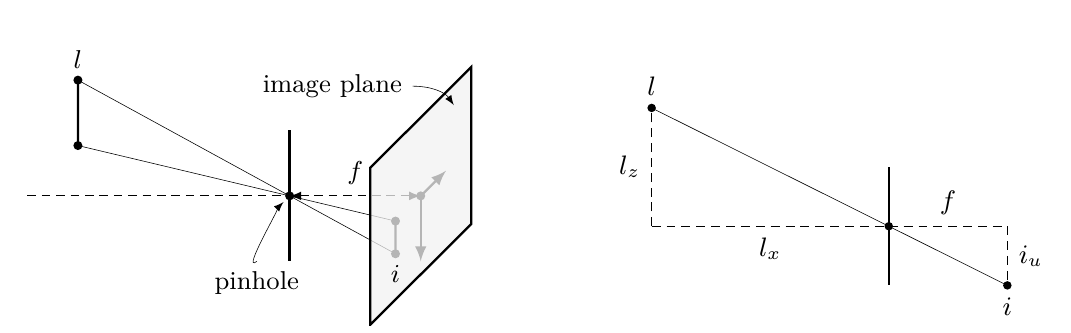
\includegraphics[width=0.9\textwidth]{figs/pinhole_camera.png}
  \caption{Pinhole camera model}
  \label{fig:pinhole_camera}
\end{figure}


\section{Planning}
The following stages are planned to be performed:
\begin{enumerate}
\item single-camera scenario - using simulated 3D world points with
  known coordinates and pinhole camera model. Here the parameters
  focal length and image center will be estimated given known
  positions of the points. Here typically knowledge about the points,
  such as inter-point distance, has to be known.
\item multi-camera scenario - using data and models same as above;
  This stage will be more challenging, since the requirement of prior
  knowledge of the points could be partially omitted. Given relative
  distances of the cameras, one can estimate positions of the points
  as well as camera parameters.
\item self-calibration algorithm -  using simulated 3D world feature
  points and lines. Exploiting the use of multiple cameras of known
  position we will remove as much a priori knowledge as possible.

\end{enumerate}

\section{Experiments and Data}

Trails have been made at Granso.

\bibliography{refs.bib}
\bibliographystyle{ieeetr}

\end{document}

%%% Local Variables:
%%% mode: latex
%%% TeX-master: t
%%% End:
